\PassOptionsToPackage{unicode=true}{hyperref} % options for packages loaded elsewhere
\PassOptionsToPackage{hyphens}{url}
%
\documentclass[12pt,]{article}
\usepackage{lmodern}
\usepackage{amssymb,amsmath}
\usepackage{ifxetex,ifluatex}
\usepackage{fixltx2e} % provides \textsubscript
\ifnum 0\ifxetex 1\fi\ifluatex 1\fi=0 % if pdftex
  \usepackage[T1]{fontenc}
  \usepackage[utf8]{inputenc}
  \usepackage{textcomp} % provides euro and other symbols
\else % if luatex or xelatex
  \usepackage{unicode-math}
  \defaultfontfeatures{Ligatures=TeX,Scale=MatchLowercase}
    \setmainfont[]{Arial}
\fi
% use upquote if available, for straight quotes in verbatim environments
\IfFileExists{upquote.sty}{\usepackage{upquote}}{}
% use microtype if available
\IfFileExists{microtype.sty}{%
\usepackage[]{microtype}
\UseMicrotypeSet[protrusion]{basicmath} % disable protrusion for tt fonts
}{}
\IfFileExists{parskip.sty}{%
\usepackage{parskip}
}{% else
\setlength{\parindent}{0pt}
\setlength{\parskip}{6pt plus 2pt minus 1pt}
}
\usepackage{hyperref}
\hypersetup{
            pdftitle={Analysis of air quality and asthma data in California, 2013-2017},
            pdfauthor={Alicia Zhao},
            pdfborder={0 0 0},
            breaklinks=true}
\urlstyle{same}  % don't use monospace font for urls
\usepackage[margin=2.54cm]{geometry}
\usepackage{longtable,booktabs}
% Fix footnotes in tables (requires footnote package)
\IfFileExists{footnote.sty}{\usepackage{footnote}\makesavenoteenv{longtable}}{}
\usepackage{graphicx,grffile}
\makeatletter
\def\maxwidth{\ifdim\Gin@nat@width>\linewidth\linewidth\else\Gin@nat@width\fi}
\def\maxheight{\ifdim\Gin@nat@height>\textheight\textheight\else\Gin@nat@height\fi}
\makeatother
% Scale images if necessary, so that they will not overflow the page
% margins by default, and it is still possible to overwrite the defaults
% using explicit options in \includegraphics[width, height, ...]{}
\setkeys{Gin}{width=\maxwidth,height=\maxheight,keepaspectratio}
\setlength{\emergencystretch}{3em}  % prevent overfull lines
\providecommand{\tightlist}{%
  \setlength{\itemsep}{0pt}\setlength{\parskip}{0pt}}
\setcounter{secnumdepth}{5}
% Redefines (sub)paragraphs to behave more like sections
\ifx\paragraph\undefined\else
\let\oldparagraph\paragraph
\renewcommand{\paragraph}[1]{\oldparagraph{#1}\mbox{}}
\fi
\ifx\subparagraph\undefined\else
\let\oldsubparagraph\subparagraph
\renewcommand{\subparagraph}[1]{\oldsubparagraph{#1}\mbox{}}
\fi

% set default figure placement to htbp
\makeatletter
\def\fps@figure{htbp}
\makeatother

\usepackage{etoolbox}
\makeatletter
\providecommand{\subtitle}[1]{% add subtitle to \maketitle
  \apptocmd{\@title}{\par {\large #1 \par}}{}{}
}
\makeatother

\title{Analysis of air quality and asthma data in California, 2013-2017}
\providecommand{\subtitle}[1]{}
\subtitle{\url{https://github.com/aliciaszhao/finalproject}}
\author{Alicia Zhao}
\date{}

\begin{document}
\maketitle

\newpage
\tableofcontents 
\newpage
\listoftables 
\newpage
\listoffigures 
\newpage

\hypertarget{rationale-and-research-questions}{%
\section{Rationale and Research
Questions}\label{rationale-and-research-questions}}

In the United States, the National Ambient Air Quality Standards from
the 1970 Clean Air Act help monitor air pollutant levels. While
significant reductions in air pollution have been made since the
standards were put in place, there are still many areas that do not meet
the standards. California, in particular, has been cited as a leader in
air pollution, with cities such as Bakersfield, Fresno, Los Angeles and
San Francisco having some of the highest recorded levels of ozone levels
in the country.

From a health perspective, exposure to higher levels of air pollutants
such as ozone (O3), nitrogen dioxide (NO2), and particulate matter
(PM2.5) is associated with reduced lung function, asthma exacerbations,
increased hospital visits, and death (Schraufnagel et al., 2019). In
fact, asthma is the leading chronic condition in children, affecting 1
in 12 children in the United States (Zahran, 2018). According to a
recent Center for Disease Control and Prevention (CDC) study, children
have higher rates of hospital and emergency department visits associated
with asthma compared to adults (Moorman et al., 2012). The health
impacts of asthma are not distributed equally among children, however.
Prevalence of asthma in children can differ by age, family history,
racial and ethnic group, and socioeconomic status (U.S. EPA, 2013).

As such, my study seeks to answer two main questions:

\begin{itemize}
\item
  \textbf{Question 1:} What are the trends of O3, NO2 and PM2.5 in some
  of the most polluted cities in California over a five-year period,
  from 2013 to 2017 ?
\item
  \textbf{Question 2:} How is asthma incidence in California impacted by
  O3 and PM2.5 levels, accounting for socioeconomic variables? Is this
  relationship different in children compared to adults?
\end{itemize}

\newpage

\hypertarget{dataset-information}{%
\section{Dataset Information}\label{dataset-information}}

\hypertarget{epa-air-quality-datasets}{%
\subsection{EPA air quality datasets}\label{epa-air-quality-datasets}}

Air quality data were collected using
\href{https://www.epa.gov/outdoor-air-quality-data/download-daily-data}{EPA's
Download Daily Data tool} (Table 1).

\begin{longtable}[]{@{}ll@{}}
\caption{Summary of selections made for daily air quality
datasets.}\tabularnewline
\toprule
Option & Selection\tabularnewline
\midrule
\endfirsthead
\toprule
Option & Selection\tabularnewline
\midrule
\endhead
Pollutant & PM2.5, Ozone and NO2\tabularnewline
Year & 2013-2017\tabularnewline
Geographic Area & California\tabularnewline
Download & Download CSV (spreadsheet)\tabularnewline
\bottomrule
\end{longtable}

The downloaded files, which were accessed on 2020-04-11, were saved in
the project folder path \texttt{./Data/Raw/Air\ quality/} as
\texttt{EPAair\_{[}Pollutant{]}\_CA\_{[}Year{]}\_raw.csv}. For example,
the O3 dataset for 2017 was saved as
\texttt{EPAair\_O3\_CA\_2017\_raw.csv}.

\hypertarget{pm2.5-dataset-content-information}{%
\subsubsection{PM2.5 dataset content
information}\label{pm2.5-dataset-content-information}}

This datset contains daily mean PM2.5 concentrations and the
corresponding air quality index (AQI) value in California over the years
2013-2017.

The number of sites and counties in the dataset varied slightly by year
(Table 2).

\begin{longtable}[]{@{}rrr@{}}
\caption{Summary of sites and counties for PM2.5
dataset.}\tabularnewline
\toprule
Year & Sites & Counties\tabularnewline
\midrule
\endfirsthead
\toprule
Year & Sites & Counties\tabularnewline
\midrule
\endhead
2013 & 149 & 52\tabularnewline
2014 & 152 & 52\tabularnewline
2015 & 151 & 52\tabularnewline
2016 & 151 & 52\tabularnewline
2017 & 152 & 51\tabularnewline
\bottomrule
\end{longtable}

\hypertarget{o3-dataset-content-information}{%
\subsubsection{O3 dataset content
information}\label{o3-dataset-content-information}}

This dataset contains daily maximum 8-hour O3 concentrations and the
corresponding air quality index (AQI) value in California over the years
2013-2017.

The number of sites and counties in the dataset varied slightly by year
(Table 3).

\begin{longtable}[]{@{}rrr@{}}
\caption{Summary of sites and counties for O3 dataset.}\tabularnewline
\toprule
Year & Sites & Counties\tabularnewline
\midrule
\endfirsthead
\toprule
Year & Sites & Counties\tabularnewline
\midrule
\endhead
2013 & 183 & 49\tabularnewline
2014 & 182 & 49\tabularnewline
2015 & 182 & 49\tabularnewline
2016 & 182 & 49\tabularnewline
2017 & 181 & 49\tabularnewline
\bottomrule
\end{longtable}

\hypertarget{no2-dataset-content-information}{%
\subsubsection{NO2 dataset content
information}\label{no2-dataset-content-information}}

This dataset contains the daily maximum 1-hour NO2 concentration and the
corresponding air quality index (AQI) value in California over the years
2013-2017.

The number of sites and counties in the dataset varied slightly by year
(Table 4).

\begin{longtable}[]{@{}rrr@{}}
\caption{Summary of sites and counties for NO2 dataset.}\tabularnewline
\toprule
Year & Sites & Counties\tabularnewline
\midrule
\endfirsthead
\toprule
Year & Sites & Counties\tabularnewline
\midrule
\endhead
2013 & 102 & 33\tabularnewline
2014 & 105 & 33\tabularnewline
2015 & 108 & 33\tabularnewline
2016 & 109 & 33\tabularnewline
2017 & 106 & 33\tabularnewline
\bottomrule
\end{longtable}

All three datasets contain 20 variables (Table 5). Variable names
without descriptions are self-explanatory.

\begin{longtable}[]{@{}ll@{}}
\caption{Summary of variables in air quality datasets.}\tabularnewline
\toprule
Variable & Description\tabularnewline
\midrule
\endfirsthead
\toprule
Variable & Description\tabularnewline
\midrule
\endhead
Date & Month/day/year\tabularnewline
Source & AQS (Air Quality System) or AirNow\tabularnewline
Site ID & A unique number within the county identifying the
site\tabularnewline
POC & Parameter Occurrence Code used to distinguish
different\tabularnewline
& instruments that measure the same parameter at the same\tabularnewline
& site\tabularnewline
Daily Mean PM2.5 Concentration &\tabularnewline
Daily Max 8-hour Ozone Concentration &\tabularnewline
Daily Max 1-hour NO2 Concentration &\tabularnewline
Units & Units for concentration\tabularnewline
Daily\_AQI\_Value & Air quality index (range 0-500)\tabularnewline
Site Name &\tabularnewline
DAILY\_OBS\_COUNT & Number of observations per day\tabularnewline
PERCENT\_COMPLETE &\tabularnewline
AQS\_PARAMETER\_CODE &\tabularnewline
AQS\_PARAMETER\_DESC &\tabularnewline
CBSA\_CODE & The FIPS code of the metropolitan area\tabularnewline
CBSA\_NAME &\tabularnewline
STATE\_CODE & The FIPS code of the state\tabularnewline
STATE &\tabularnewline
COUNTY\_CODE & The FIPS code of the county\tabularnewline
COUNTY &\tabularnewline
SITE\_LATITUDE &\tabularnewline
SITE\_LONGITUDE &\tabularnewline
\bottomrule
\end{longtable}

\begin{longtable}[]{@{}ll@{}}
\caption{Air quality index (AQI) values and corresponding levels of
health concern.}\tabularnewline
\toprule
AQI.Values & Levels.of.Heath.Concern\tabularnewline
\midrule
\endfirsthead
\toprule
AQI.Values & Levels.of.Heath.Concern\tabularnewline
\midrule
\endhead
0-50 & Good\tabularnewline
51-100 & Moderate\tabularnewline
101-150 & Unhealthy for Sensitive Groups\tabularnewline
151-200 & Unhealthy\tabularnewline
201-300 & Very unhealthy\tabularnewline
301-500 & Hazardous\tabularnewline
\bottomrule
\end{longtable}

\hypertarget{data-wrangling}{%
\subsubsection{Data wrangling}\label{data-wrangling}}

Air quality datasets for different years were combined using
\texttt{rbind} to form one dataset for each pollutant.

The following columns were selected:

\begin{itemize}
\tightlist
\item
  \textbf{Date}\\
\item
  \textbf{Site.ID}\\
\item
  \textbf{Daily.Max.1.hour.NO2.Concentration}\\
\item
  \textbf{DAILY\_AQI\_VALUE}\\
\item
  \textbf{Site.Name}\\
\item
  \textbf{COUNTY}
\end{itemize}

Additionally, columns for \textbf{Month} and \textbf{Year} were added
using the \textbf{Date} column.

\hypertarget{asthma-datasets}{%
\subsection{Asthma datasets}\label{asthma-datasets}}

Asthma data were collected using
\href{https://trackingcalifornia.org/asthma/query}{Tracking California's
Asthma Data Query tool} (Table 7).

\begin{longtable}[]{@{}ll@{}}
\caption{Summary of selections made for daily asthma
datasets.}\tabularnewline
\toprule
Option & Selection\tabularnewline
\midrule
\endfirsthead
\toprule
Option & Selection\tabularnewline
\midrule
\endhead
Type of event & Emergency department visits due to asthma\tabularnewline
Age sub-group & Age 0-17, AGe 18 \& over\tabularnewline
Year & 2013-2017\tabularnewline
How event is measured & Age-adjusted rates per 10,000\tabularnewline
Race/ethnicity & All races/ethnicities\tabularnewline
Gender/sex & Both sexes\tabularnewline
Type of information & Conventional\tabularnewline
Type of geography & Zip codes\tabularnewline
\bottomrule
\end{longtable}

The downloaded files, which were accessed on 2020-04-12, were saved in
the project folder path \texttt{./Data/Raw/Asthma/} as
\texttt{TrackingCA\_Asthma\_ERVisits\_{[}Age\ Group{]}\_{[}Year{]}\_raw.csv}.
For example, the dataset for adults in 2013 was saved as
\texttt{TrackingCA\_Asthma\_ERVisits\_Adults\_2013\_raw.csv}.

\hypertarget{adult-asthma-dataset-content-information}{%
\subsubsection{Adult asthma dataset content
information}\label{adult-asthma-dataset-content-information}}

This dataset contains the annual rates of asthma-related ER visits for
adults in California over the years 2013-2017.

\hypertarget{children-asthma-dataset-content-information}{%
\subsubsection{Children asthma dataset content
information}\label{children-asthma-dataset-content-information}}

This dataset contains the annual rates of asthma-related ER visits for
children in California over the years 2013-2017.

Both datasets contain 2 variables. Variable names without descriptions
are self-explanatory.

\begin{longtable}[]{@{}ll@{}}
\caption{Summary of variables in asthma datasets.}\tabularnewline
\toprule
Variable & Description\tabularnewline
\midrule
\endfirsthead
\toprule
Variable & Description\tabularnewline
\midrule
\endhead
Zip code &\tabularnewline
Incidence & Age-adjusted rate of emergency department
visits\tabularnewline
& due to asthma per 10,000 California residents\tabularnewline
\bottomrule
\end{longtable}

\hypertarget{data-wrangling-1}{%
\subsubsection{Data wrangling}\label{data-wrangling-1}}

A \textbf{Year} column was added to all asthma datasets. Datasets for
2013-2017 were combined using \texttt{rbind} to form one dataset for
each age group (Adults, Children).

Since the asthma datasets provide only zip code information but not
county information, an online search was done to find zip codes and
their corresponding counties in California. This information was scraped
into a data frame. This dataframe was then combined with the adult
dataset and the children dataset using \texttt{left\_join}. The
incidence rates were then grouped by county and the average incidence
rate for each county was calculated.

Finally, adult and children asthma datasets were combined using
\texttt{full\_join}.

\hypertarget{demographics-dataset}{%
\subsection{Demographics dataset}\label{demographics-dataset}}

Demographic data were collected from
\href{https://www.countyhealthrankings.org/app/california/2019/downloads}{County
Health Rankings \& Roadmaps}.

Since demographics are assumed to remain somewhat constant over the
five-year period, only one dataset was chosen. The 2019 dataset, which
uses data published in 2017, was chosen.

The xls file, was accessed on 2020-04-12, was saved in the project
folder path \texttt{./Data/Raw/Demographics/} as
\texttt{CountyHealthRankings\_CA\_2019\_raw.xls}. Since there multiple
tabs in the xls file, relevant information from the file was taken and
converted into a csv file.The csv file was saved as
\texttt{CountyHealthRankings\_CA\_2019\_filtered\_raw.csv}.

The following information is contained in the dataset:\\
* \textbf{FIPS}\\
* \textbf{State}\\
* \textbf{County}\\
* \textbf{Median Household Income}\\
* \textbf{Population}\\
* \textbf{Percent African American}\\
* \textbf{Percent Rural}\\
* \textbf{Percent Smokers}

\newpage

\hypertarget{exploratory-analysis}{%
\section{Exploratory Analysis}\label{exploratory-analysis}}

\hypertarget{air-quality-datasets}{%
\subsection{Air quality datasets}\label{air-quality-datasets}}

In examining the air quality index (AQI) values for the three pollutants
across all sites, there is not much temporal variation (Figure 1).
However, the frequency distrbution does differ by pollutant. NO2
generally has lower AQI values, which aggregate well below 50, the
cut-off number for the ``Good'' air quality range. O3 and PM2.5 have
higher AQI values, which concentrate closer to 50, and also contain more
values that are above 50.

\begin{figure}
\centering
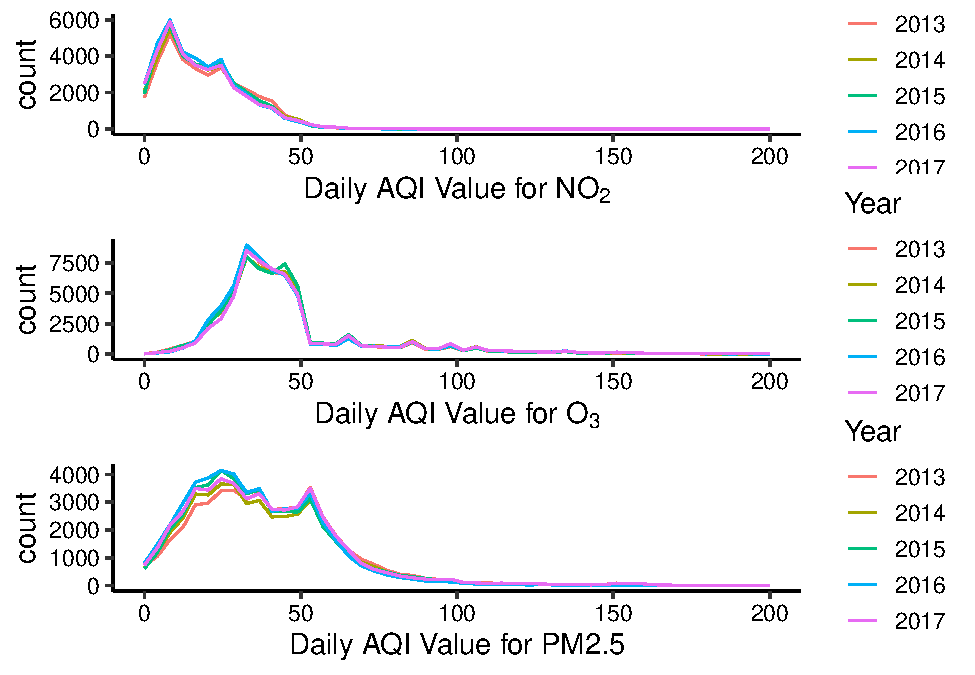
\includegraphics{FinalProject_AliciaZhao_files/figure-latex/unnamed-chunk-9-1.pdf}
\caption{Frequency of daily AQI values in California from 2013 to 2017.}
\end{figure}

\newpage

Among the four target sites (Bakersfield, Fresno, Los Angeles and San
Francisco), Bakersfield appears to have higher AQI values than the other
sites across all pollutants (Figure 2). In contrast, San Francisco
generally has lower AQI values compared to the other sites. Although AQI
values for NO2 stay below the ``Unhealthy for sensitive populations''
range (denoted by the dashed line) for all sites, the AQI values for O3
and PM2.5 are generally in this range.

\begin{figure}
\centering
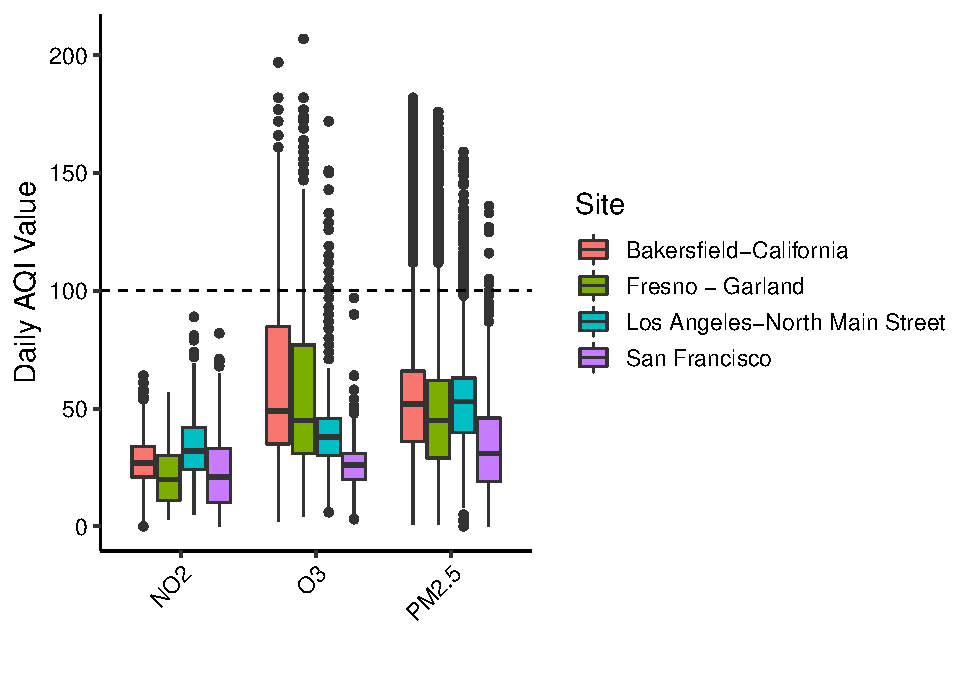
\includegraphics{FinalProject_AliciaZhao_files/figure-latex/unnamed-chunk-10-1.pdf}
\caption{Boxplots of daily AQI values in four key sites from 2013 to
2017.}
\end{figure}

\newpage

\hypertarget{asthma-datasets-1}{%
\subsection{Asthma datasets}\label{asthma-datasets-1}}

In examining the asthma-related ER visits for adults and children across
58 counties in California, children appear to have more asthma-related
ER visits than adults (Figure 3). Distributions for both age groups show
a right skew.

\begin{figure}
\centering
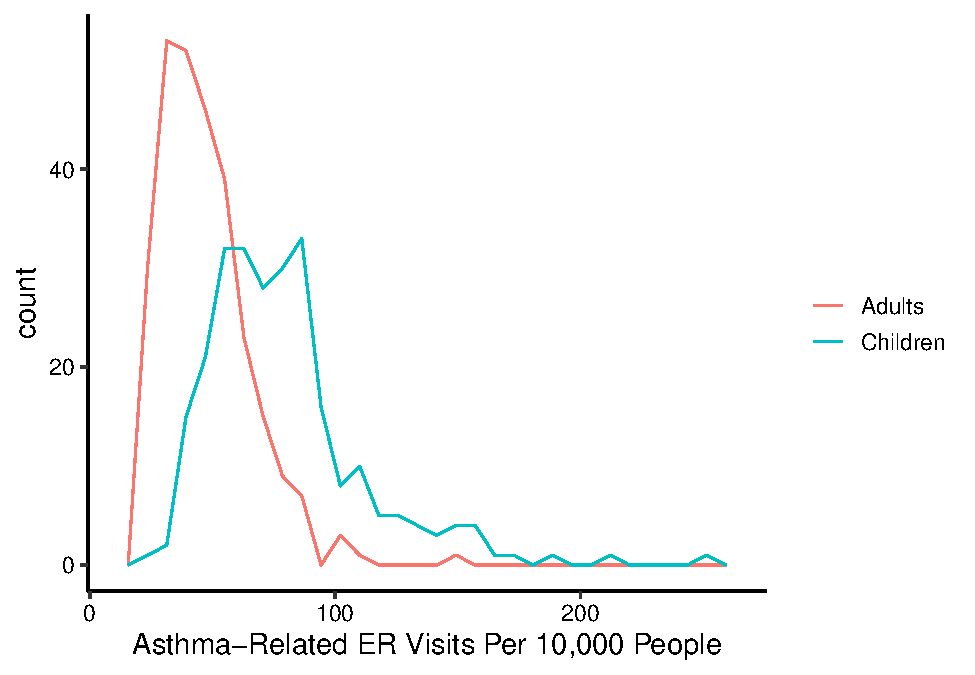
\includegraphics{FinalProject_AliciaZhao_files/figure-latex/unnamed-chunk-12-1.pdf}
\caption{Frequency of asthma-related ER visitation rates for children
and adults in California from 2013 to 2017.}
\end{figure}

\newpage

\hypertarget{demographics-dataset-1}{%
\subsection{Demographics dataset}\label{demographics-dataset-1}}

In examining demographics for 52 counties in California, counties
generally have a low percentage of African American residents and a much
higher percentage of Hispanic residents; a median household income
clustering between 40,000 and 75,000; and more urban areas than rural
areas (Figure 4).

\begin{figure}
\centering
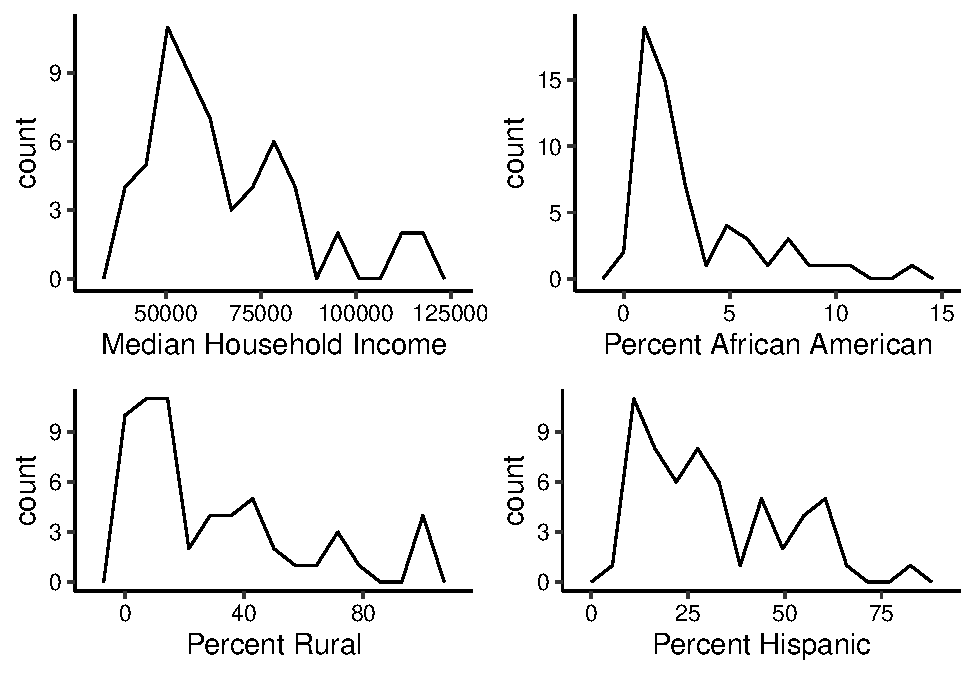
\includegraphics{FinalProject_AliciaZhao_files/figure-latex/unnamed-chunk-14-1.pdf}
\caption{Frequency of median household income, percent African American,
percent rural, and percent Hispanic across counties in California from
2013 to 2017.}
\end{figure}

\newpage

\hypertarget{analysis}{%
\section{Analysis}\label{analysis}}

\hypertarget{time-series-analysis}{%
\subsection{Time Series Analysis}\label{time-series-analysis}}

The time series analysis method was used to determine trends of O3, NO2
and PM2.5 in some of the most polluted cities in California from 2013 to
2017 (Figures 5-8). The four sites chosen were: Bakersfield, Fresno, Los
Angeles and San Francisco.

The dashed lines in the figures separate the AQI categories into
\textbf{`Good'}, \textbf{`Moderate'}, and \textbf{`Unhealthy for
sensitive groups'}. San Francisco appears to have the lowest levels of
pollution, whereas O3 and PM2.5 levels for both Bakersfield and Fresno
have reached the unhealthy level.

In performing seasonal Mann-Kendall tests to these time series, it was
observed that there are some trends for the pollutants beyond seasonal
trends.

\newpage

\hypertarget{bakersfield}{%
\subsubsection{Bakersfield}\label{bakersfield}}

There is a decreasing overall trend for NO2 (seasonal Mann-Kendall, z=
-2.41, p-value = 0.016), a decreasing overall trend for PM2.5 (seasonal
Mann-Kendall, z = -3.46, p-value \textless{} 0.001) and no significant
trend for O3 beyond seasonal trends over the period 2013-2017.

\begin{figure}
\centering
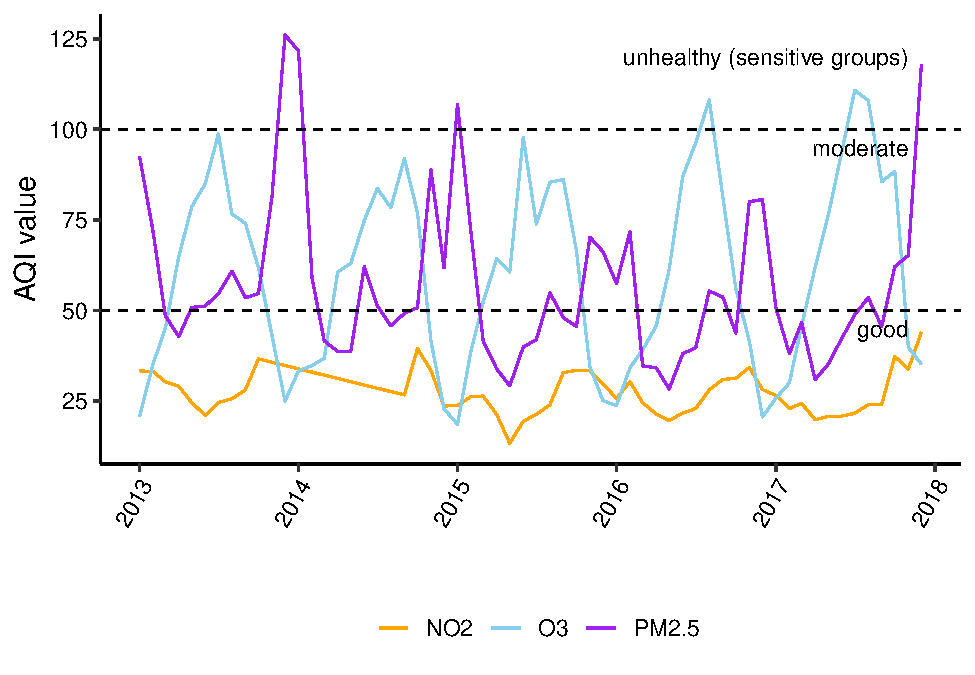
\includegraphics{FinalProject_AliciaZhao_files/figure-latex/unnamed-chunk-17-1.pdf}
\caption{Time series analysis of monthly AQI values in Bakersfield, CA
from 2013 to 2017.}
\end{figure}

\newpage

\hypertarget{fresno}{%
\subsubsection{Fresno}\label{fresno}}

There is no significant trend for NO2, O3, or PM2.5 beyond seasonal
trends over the period 2013-2017.

\begin{figure}
\centering
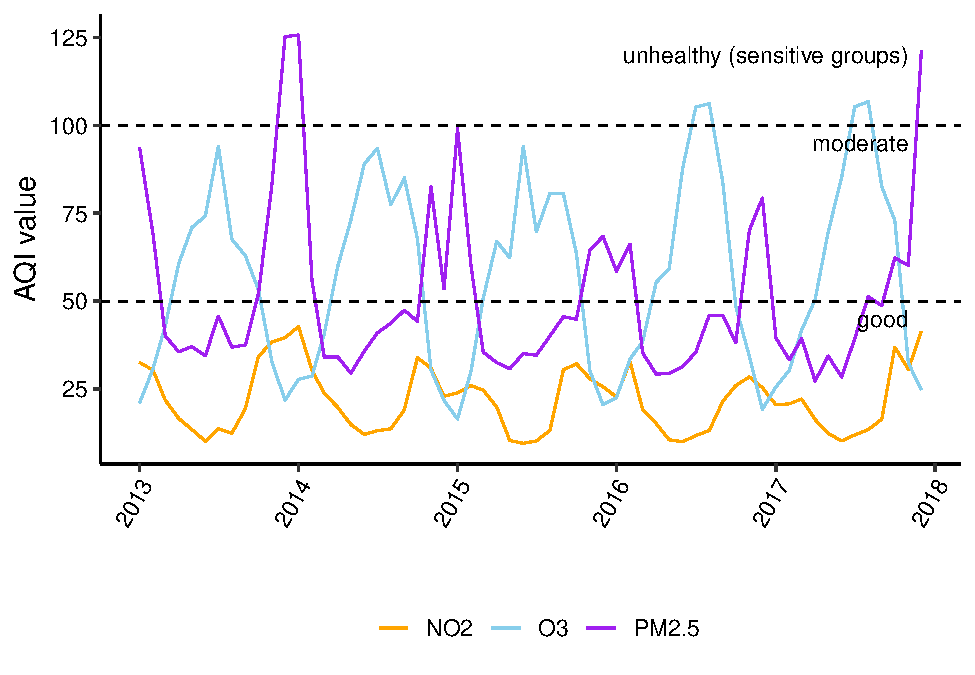
\includegraphics{FinalProject_AliciaZhao_files/figure-latex/unnamed-chunk-18-1.pdf}
\caption{Time series analysis of monthly AQI values in Fresno, CA from
2013 to 2017.}
\end{figure}

\newpage

\hypertarget{los-angeles}{%
\subsubsection{Los Angeles}\label{los-angeles}}

There is a no significant trend for NO2 beyond seasonal trends, an
overall increasing trend for O3 (seasonal Mann-Kendall, z = 3.18,
p-value =.0001), and an overall decreasing trend and a decreasing trend
in April for PM2.5 ( seasonal Mann-Kendall, z = -2.05, p-value = 0.040;
z = -2.205, p-value= 0.027) over the period 2013-2017.

\begin{figure}
\centering
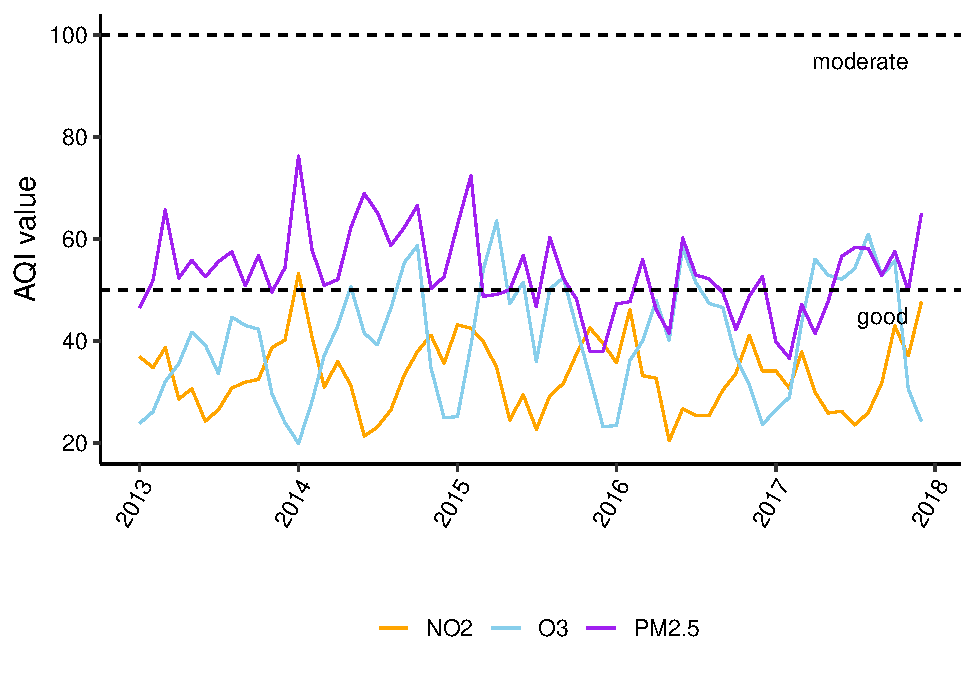
\includegraphics{FinalProject_AliciaZhao_files/figure-latex/unnamed-chunk-19-1.pdf}
\caption{Time series analysis of monthly AQI values in Los Angeles, CA
from 2013 to 2017.}
\end{figure}

\newpage

\hypertarget{san-francisco}{%
\subsubsection{San Francisco}\label{san-francisco}}

There is an overall decreasing trend for NO2 (seasonal Mann-Kendall, z =
-2.192, p-value = 0.028), and no significant trend for O3 or PM2.5 over
the period 2013-2017.

\begin{figure}
\centering
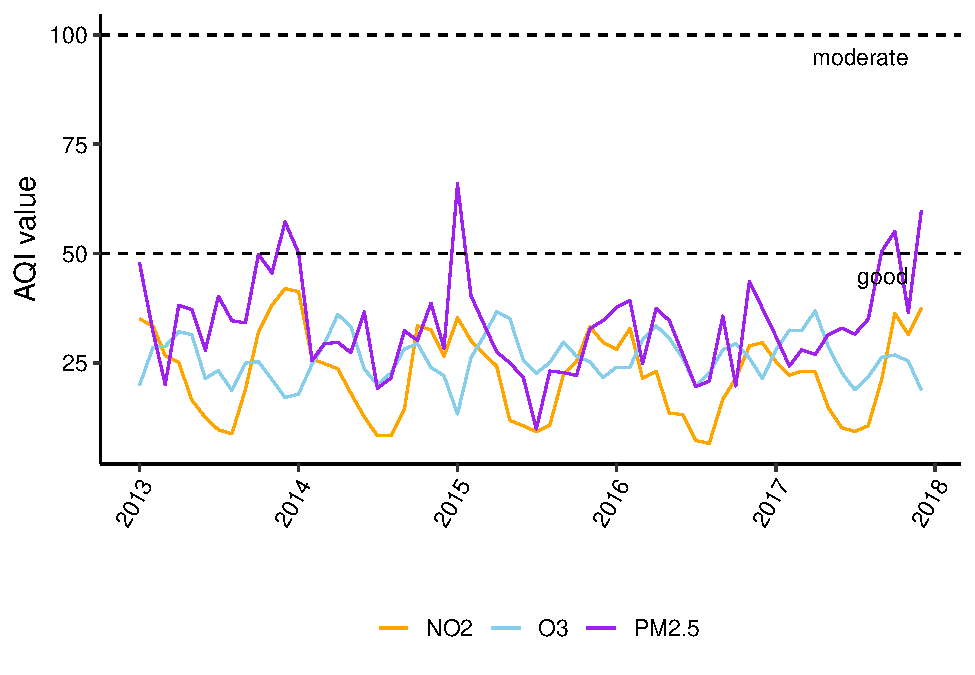
\includegraphics{FinalProject_AliciaZhao_files/figure-latex/unnamed-chunk-20-1.pdf}
\caption{Time series analysis of monthly AQI values in San Francisco, CA
from 2013 to 2017.}
\end{figure}

\newpage

\hypertarget{general-linear-model}{%
\subsection{General Linear Model}\label{general-linear-model}}

The general linear model (GLM) method was used to answer how asthma
incidence in children and adults is impacted by O3 and PM2.5 levels and
socioeconomic variables.Data were evaluated on a county-level across the
years 2013 to 2017.

\hypertarget{dependent-variables}{%
\subsubsection{Dependent variables}\label{dependent-variables}}

The dependent variable is asthma incidence, measured by using
age-adjusted asthma-related ER visitation rates per 10,000 residents.
This rate was evaluated separately for adults and children.

\hypertarget{explanatory-variables}{%
\subsubsection{Explanatory variables}\label{explanatory-variables}}

The explanatory variables are:\\
* \textbf{Annual average O3 AQI value}\\
* \textbf{Annual average PM2.5 AQI value}\\
* \textbf{Median household income}\\
* \textbf{Percent African American}\\
* \textbf{Percent Hispanic}\\
* \textbf{Percent rural}\\
* \textbf{Percent smokers}

\textbf{O3} and \textbf{PM2.5} were included to evaluate the impact of
air quality on asthma incidence. \textbf{NO2} was not chosen because as
the exploratory analysis showed, NO2 levels are not as high as O3 and
PM2.5 levels, and also there were more missing data for NO2.

Additionally, a few demographic variables were also evaluated.
\textbf{Median household income} was chosen to account for socioeconomic
factors. \textbf{Percent African American} and \textbf{Percent Hispanic}
were chosen to account for racial factors. \textbf{Percent rural} was
chosen to account for differences in air quality and healthcare access.
\textbf{Percent smokers} was chosen to account for other health factors
that could impact asthma.

\newpage

\hypertarget{asthma-incidence-in-children}{%
\subsubsection{Asthma incidence in
children}\label{asthma-incidence-in-children}}

A multiple linear regression was run to predict asthma-related emergency
room visitation rates in children while accounting for the explanatory
variables described previously.

The most parsimonious model includes the variables \textbf{O3},
\textbf{percent African American}, \textbf{percent Hispanic},
\textbf{percent rural} and \textbf{percent smokers} (linear regression,
adjusted R2 = .66, df = 159 and p-value = \textless{}.001).

According to this model, holding all other variables constant, for every
unit increase in the AQI for O3, the ER visitiation rate decreases by
.67. For every percent increase in African American populations, ER
visitation rate increases by 5.3. For every percent increase in Hispanic
populations, the ER visitation rate increase by 1.2. For every percent
increase in rural areas, the ER visitation rate increases by 1.2. For
every percent increase in smokers, the ER visitations rate increases by
2.9.

\begin{figure}
\centering
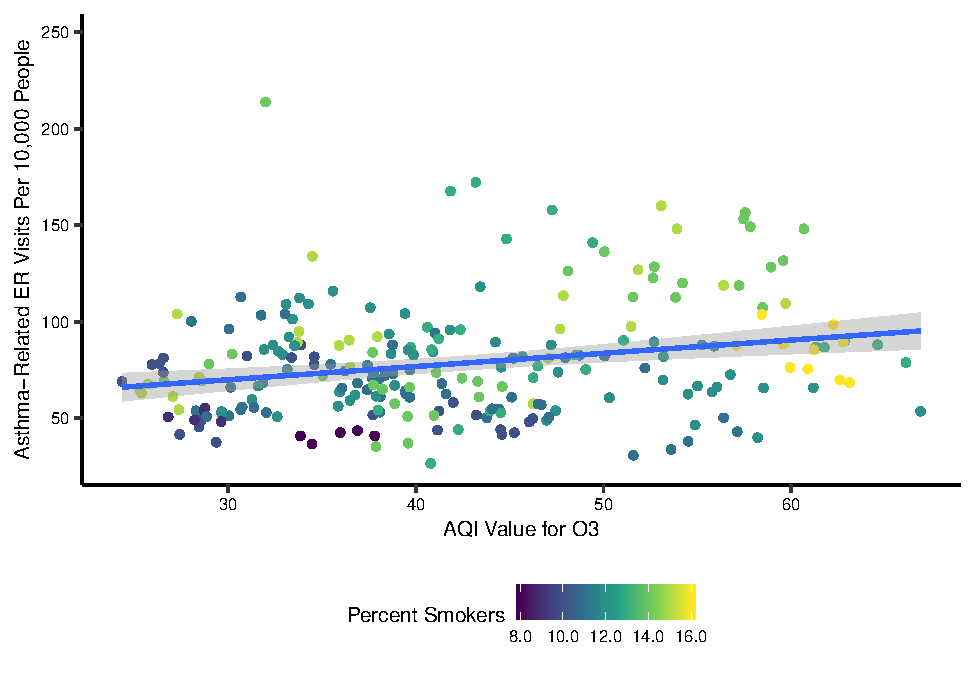
\includegraphics{FinalProject_AliciaZhao_files/figure-latex/unnamed-chunk-22-1.pdf}
\caption{Annual average O3 AQI values, percent smokers, and
asthma-related ER visitation rates for children across 52 counties in
California from 2013 to 2017.}
\end{figure}

\begin{figure}
\centering
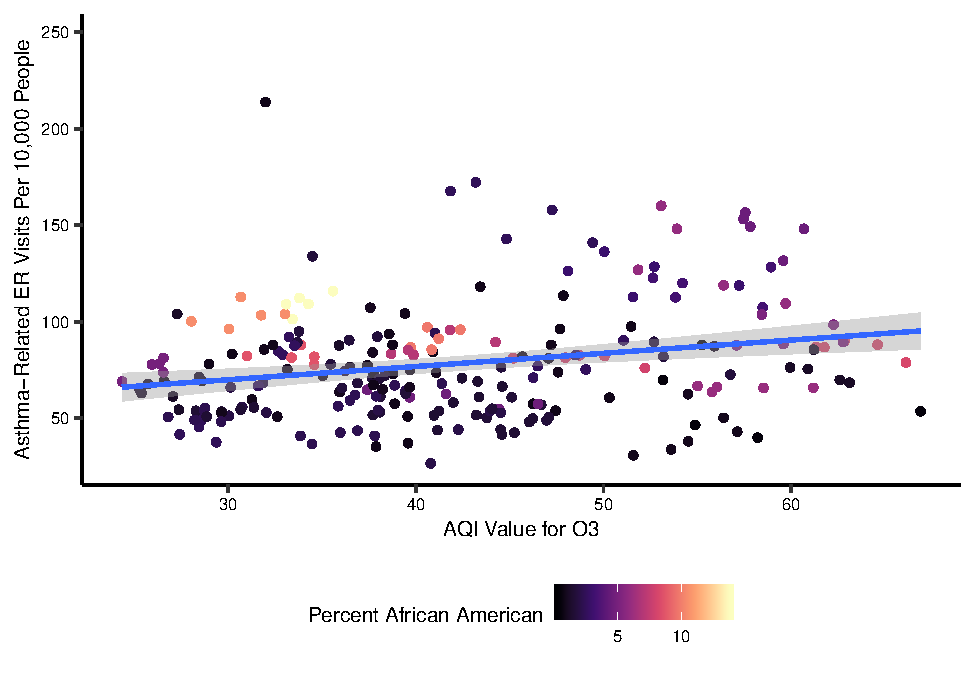
\includegraphics{FinalProject_AliciaZhao_files/figure-latex/unnamed-chunk-23-1.pdf}
\caption{Annual average O3 AQI values, percent African American, and
asthma-related ER visitation rates for children across 52 counties in
California from 2013 to 2017.}
\end{figure}

\newpage

\hypertarget{asthma-incidence-in-adults}{%
\subsubsection{Asthma incidence in
adults}\label{asthma-incidence-in-adults}}

A multiple linear regression was run to predict asthma-related emergency
room visitation rates in adults while accounting for the explanatory
variables described previously.

The most parsimonious model includes the variables \textbf{O3},
\textbf{percent African American} and \textbf{percent smokers} (linear
regression, adjusted R2 =.59, df = 161, p-value \textless{}.001).

According to this model, holding all other variables constant, for every
unit increase in the AQI for O3, the ER visitiation rate decreases by
.41. For every percent increase in African American populations, the ER
visitation rate increases by 2.4. For every percent increase in smokers,
the ER visitations rate increases by 5.3.

\begin{figure}
\centering
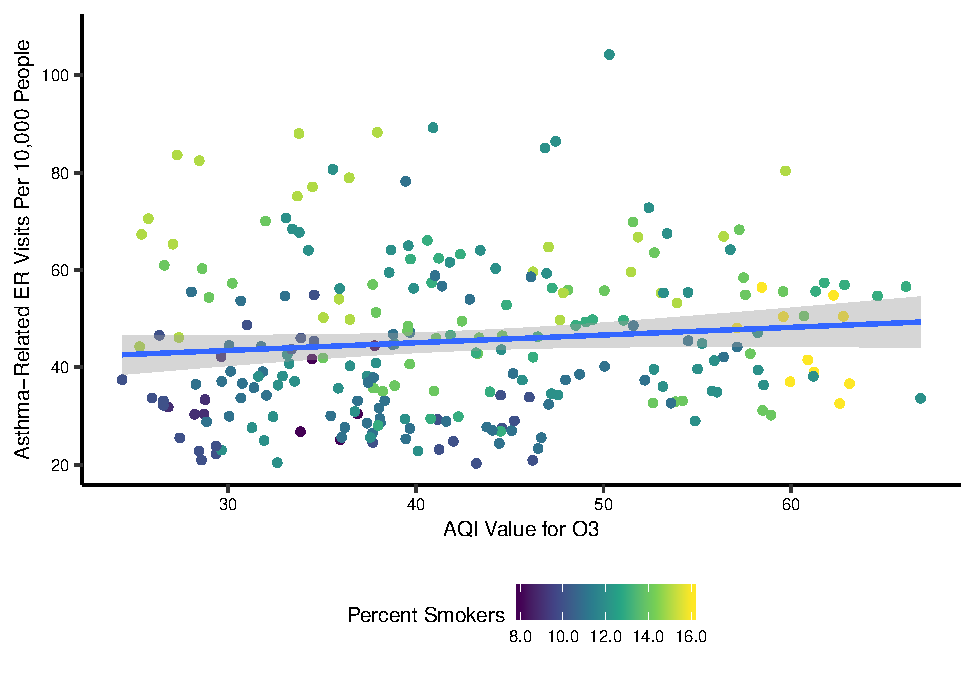
\includegraphics{FinalProject_AliciaZhao_files/figure-latex/unnamed-chunk-24-1.pdf}
\caption{Annual average O3 AQI values, percent smokers, and
asthma-related ER visitation rates for adults across 52 counties in
California from 2013 to 2017}
\end{figure}

\begin{figure}
\centering
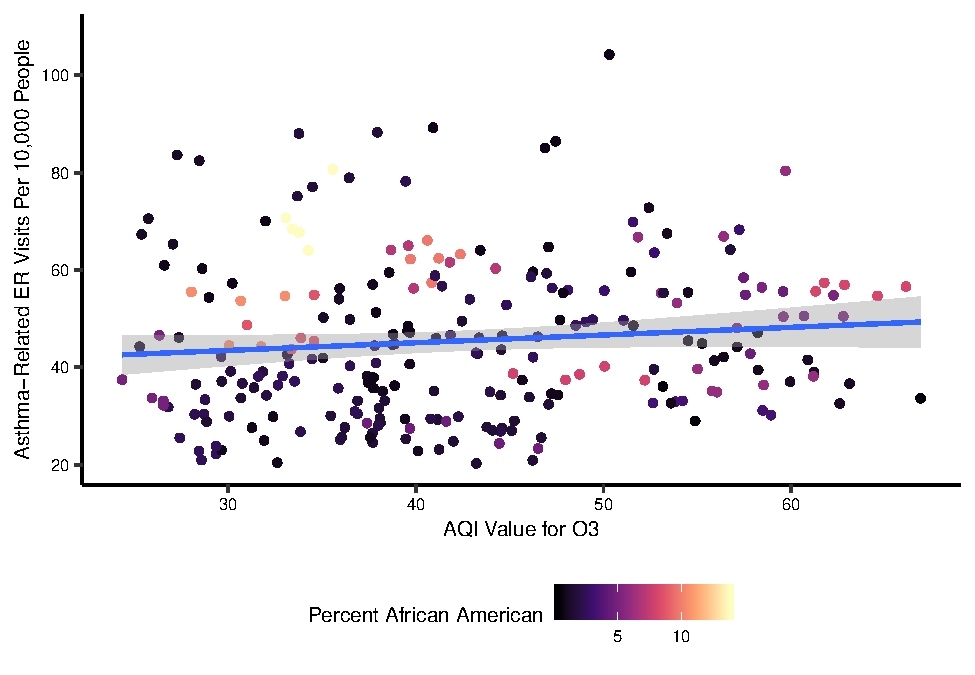
\includegraphics{FinalProject_AliciaZhao_files/figure-latex/unnamed-chunk-25-1.pdf}
\caption{Annual average O3 AQI values, percent African American, and
asthma-related ER visitation rates for adults across 52 counties in
California from 2013 to 2017}
\end{figure}

\newpage

\hypertarget{summary-and-conclusions}{%
\section{Summary and Conclusions}\label{summary-and-conclusions}}

\hypertarget{question-1-what-are-the-trends-of-o3-no2-and-pm2.5-in-some-of-the-most-polluted-cities-in-california-over-a-five-year-period-from-2013-to-2017}{%
\subsection{\texorpdfstring{\textbf{Question 1:} What are the trends of
O3, NO2 and PM2.5 in some of the most polluted cities in California over
a five-year period, from 2013 to 2017
?}{Question 1: What are the trends of O3, NO2 and PM2.5 in some of the most polluted cities in California over a five-year period, from 2013 to 2017 ?}}\label{question-1-what-are-the-trends-of-o3-no2-and-pm2.5-in-some-of-the-most-polluted-cities-in-california-over-a-five-year-period-from-2013-to-2017}}

The time series analysis from this study suggest that the most part,
there is either no trend or a decreasing trend for all pollutants across
the sites, which is encouraging to find. The exception is O3 in LA,
which has shown an increasing trend. However, this is not too much of a
concern, as ozone levels are only bordering the `Moderate' range but
mostly still in the `Good' range.

\hypertarget{question-2-how-is-asthma-incidence-in-california-impacted-by-o3-and-pm2.5-levels-accounting-for-socioeconomic-variables-is-this-relationship-different-in-children-compared-to-adults}{%
\subsection{\texorpdfstring{\textbf{Question 2:} How is asthma incidence
in California impacted by O3 and PM2.5 levels, accounting for
socioeconomic variables? Is this relationship different in children
compared to
adults?}{Question 2: How is asthma incidence in California impacted by O3 and PM2.5 levels, accounting for socioeconomic variables? Is this relationship different in children compared to adults?}}\label{question-2-how-is-asthma-incidence-in-california-impacted-by-o3-and-pm2.5-levels-accounting-for-socioeconomic-variables-is-this-relationship-different-in-children-compared-to-adults}}

Findings from this study suggest that asthma incidence in both children
and adults are impacted by \textbf{O3}, \textbf{percent African
Americans} and \textbf{percent smokers} in each county. However,
incidence in children is more impacted by race (such as \textbf{percent
African American} and \textbf{percent Hispanic}) and \textbf{percent
rural} in each county when compared to incidence in adults. On the other
hand, asthma incidence in adults is more sensitive to \textbf{percent
smokers} in each county.

Surprisingly, PM2.5 was not found to be a significant variable in our
models. Additionally, although O3 was a significant variable, it has a
slightly inverse relationship with asthma incidence, which is contrary
to what was expected. One explanation is that because air pollution
levels are generally in the healthy range in California, their impacts
on asthma incidence are negligible when compared to the impacts of
socioeconomic and racial variables. There also are likely temporal,
spatial and other types of variables which were left out in the model,
which can cause omitted variable bias.

Based on our results from 2013-2017, California counties with a higher
percentage of African American populations and a higher percentage of
smokers are more likely to have higher asthma incidence rates in both
children and adults. These results reveal that policies targeting better
health outcomes may not achieve desired results by only reducing air
pollution. Pre-existing disparities associated with socioeconomic and
racial status may play a larger role in impacting asthma incidence, and
should be addressed in conjunction with air quality policies.

\newpage

\hypertarget{references}{%
\section{References}\label{references}}

Moorman JE, Akinbami LJ, Bailey CM, Zahran HS, King ME, Johnson CA, et
al.~National surveillance of asthma: United States, 2001--2010. (2012).
Vital Health Stat 3 (35):1--58.

Schraufnagel, D.E. et al. (2019). Air pollution and noncommunicable
diseases: a review by the forum of International Respiratory Societies'
Environmental Committee, part 1. Chest. 155(2), pp.409-416.

U.S. EPA. (2013). America's Children and the Environment, Third Edition.

Zahran, H.S., Bailey, C.M., Damon, S.A., Garbe, P.L. \& Breysse, P.N.
Vital signs: Asthma in children -- United States, 2001-2016. (2018).
Morb Mortal. Wkly Rep.~67, pp.149-155.

\end{document}
